\documentclass[11pt]{article}

\usepackage[a4paper,
            bindingoffset=0.5cm,
            left=3cm,
            right=3cm,
            top=3cm,
            bottom=4cm,
            footskip=1.5cm]{geometry}
            
%
\usepackage[T1]{fontenc}
\usepackage{graphicx}
\usepackage{enumitem}
\usepackage{blindtext}
\usepackage{float}
%

\setcounter{secnumdepth}{3}

%%%%%%%%%%%%%%%%%%%%%
\title{\textbf{Critical Systems Lab - MESCC\\ Water Pumping Automated System}}
\date{ISEP, January 2024}
\author{Ricardo Mendes\\ 1201779
\and Arthur Gerbelli\\ 1220201}
%%%%%%%%%%%%%%%%%%%%%

\begin{document}

\maketitle              
\newpage
\tableofcontents
\newpage

%
\section{Introduction}

This document is a follow-up of the previous work.

It takes into account the feedback received during the last presentation and also the current objectives of the exercise.

%%%
\section{Requirement Specification}

%%%
\subsection{Problem Domain - Update}

%%%
\subsubsection{Notes on the previous work}

Although not mentioned on the assignment, we choosed to add some changes to the Stakeholder Needs that are paramount to understand the next chapters.




SN-1.3 Every WPS will have two pumps mainly for redundancy purpose.

SN-1.4 To improve the systems performance, and given that we have one unused water pump, this pump should only be used when the water level is above medium.

SN-1.5 In case that only one water pump is operational, the max capacity of the WPS should be lower.

[adicionar ao papyrus]


Show traceability (system context and system subsystems)

%%%
\subsection{Solution Domain}






Model the reality

Specify how sensor works




%%%
\subsubsection{System Requirements}

\begin{enumerate}[leftmargin=4em, font=\small, label=\textbf{SR-\arabic*}]
	\setlength\itemsep{.5em}
	\item 
		\begin{enumerate}[leftmargin=1.5em, font=\small, label=\textbf{.\arabic*:}]
		\setlength\itemsep{0em}
		\item While the water level is above the minimum level, WPS shall have a pump working.
		\item When the water level is below minimum level, WPS shall have all pumps stopped.
		\item If the water level is above the maximum level, then the WPS shall trigger an alarm at the Remote Status Station (RSS).
		\item A second pump shall be turned on only when the water level is above 2/3 the maximum water level.
		\item When only one pump is available, the maximum water level shall be reduced to 2/3.
		\end{enumerate}
	\item
		\begin{enumerate}[leftmargin=1.5em, font=\small, label=\textbf{.\arabic*:}]
		\setlength\itemsep{0em}
		\item The status of all WPS shall be displayed on all RSS.
		\item If the alarm is ON, the button in the RSS shall only disable it.
		\end{enumerate}
	\item The status of all WPS shall be visible on a web page.

\end{enumerate}

%%%
\subsubsection{System Structure}

\begin{figure}[H]
  \centering
  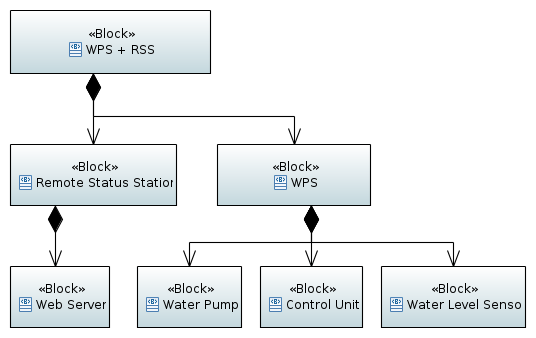
\includegraphics[width=300px]{../diagrams/system-structure.png}
  \caption{System Structure Diagram}
  \label{fig:System Structure Diagram}
\end{figure}

\newpage

%%%
\subsubsection{System Behavior}

We adopted the \textit{Mealy Finite State Machine} to describe the behavior of the WPS.

The only input to the machine is the current water level. The state of the machine changes according to these values.

There are two main states are ON and OFF, corresponding to water being or not pumped outside the well. If the water level in above the minimum, a water pump must be working (ON LOW). Depending on the levels above minimum, we can have a second pump working with (ON HIGH) or without (ON ALERT) an alert being triggered.

The state machine, beneath, models this behavior.

\begin{figure}[H]
  \centering
  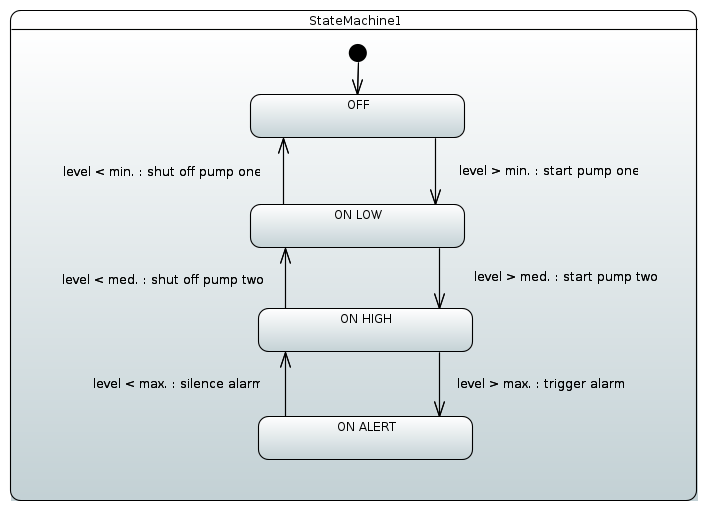
\includegraphics[width=300px]{../diagrams/state-machine-wps.png}
  \caption{State Machine}
  \label{fig:State Machine}
\end{figure}


%%%
%%%
%%%
\subsection{Analysis of safety and reliability}

Given that we are dealing with a critical system, the analysis of safety and reliability as bigger impact on the implementation of the solution.

\begin{enumerate}[leftmargin=4em, font=\small, label=\textbf{H-\arabic*:}]
	\setlength\itemsep{.5em}
	\item 
		\begin{itemize}
		\setlength\itemsep{0em}
        		\item \textbf{Description:} One of the pumps stops working.
		\item Cause: Mechanical problem.
    		\item Effect: Lost of redundancy and reduction of system performance.
    		\item \textbf{Mitigation:} Reduce the maximum water level to 2/3 and trigger alarm.
		\end{itemize}
	\item 
		\begin{itemize}
		\setlength\itemsep{0em}
    		\item \textbf{Description:} The two level sensors give contradictory readings, i.e. one above max and one below min.
		\item Cause: Sensor malfunction, connection issues.
    		\item Effect: Inappropriate system behavior. 
    		\item \textbf{Mitigation:} Choose a worst case or compare with the last reading to find the fault. Always trigger the alarm.
		\end{itemize}
	\item 
		\begin{itemize}
		\setlength\itemsep{0em}
    		\item \textbf{Description:} Power shortage.
		\item Cause: Multiple causes
    		\item Effect: Complete failure of the system.
    		\item \textbf{Mitigation:} RSS with independente power supply and trigger alarm.
		\end{itemize} 
	\item 
		\begin{itemize}
		\setlength\itemsep{0em}
    		\item \textbf{Description:} Both pumps stopped working.
		\item Cause: Mechanical problem.
    		\item Effect: Complete failure of the system.
    		\item \textbf{Mitigation:} Trigger alarm.
		\end{itemize} 
	\item 
		\begin{itemize}
		\setlength\itemsep{0em}
    		\item \textbf{Description:} RSS are not getting information from WPS.
		\item Cause: Connection issues or Messagem broker stoped working.
    		\item Effect: Unknown status of the system.
    		\item \textbf{Mitigation:} Implement a cluter of MQTT Brokers or remove this single point of failure by adopting DDS.
		\end{itemize} 
	\item 
		\begin{itemize}
		\setlength\itemsep{0em}
    		\item \textbf{Description:} RSS stops working.
		\item Cause: Malfunction.
    		\item Effect: Unknown WPS status.
    		\item \textbf{Mitigation:} Have redundancy by having multiple RSS and each one displaying all statuses from all WPS.
		\end{itemize} 
	\item 
		\begin{itemize}
		\setlength\itemsep{0em}
    		\item \textbf{Description:} A pump doesn't turn OFF when the water level in bellow minimum.
			\item Cause: Mechanical problem.
    		\item Effect: Pump overheating and complete failure.
    		\item \textbf{Mitigation:} Trigger alarm.
		\end{itemize} 
\end{enumerate}

Most of the hazards listed could be handled as non-functional requirements. Because of that, a more detailed description of some of them is needed.
\\[12pt]
\textbf{H-1} and \textbf{H-4} touches on the redundancy of the water pumps. Because having an unused water pump would mean a reduced performance of the system, we choose to use the two pumps even when the system is healthy. The second pump is only used when the water level is high. If, for some reason, one of the pumps is not working, the system will reduce the max capacity of the well and trigger an alarm to alert the maintenance team.
\\[12pt]
\textbf{H-2} is interesting because introduces a problem that cannot be answered with a reliable voting system. If the reading of both sensor are too unequal, there must be a way to distinguish between the wrong and the correct data. There are three possible ways to deal with the issues: choose a master and a slave sensor, retain the previous input and compare it with the current one, or choose the worst case.
\\[12pt]
\textbf{H-3} and \textbf{H-6} illustrates the importance of the RSS. During a localized power shortage on the well, the RSS should not be affected and so, still be able to alert the maintenance team. Having two RSS in the building also assures redundancy, specially if they have separated power supplies.
\\[12pt]
\textbf{H-5} is sensible to a special limitation of having only one system dealing with the main communication. A single MQTT broker is also a single point of failure that could jeopardize the whole system. Having a cluster of brokers or using a middleware like DDS is a way to mitigate or even remove completely this risk.

\newpage
%%%
\section{Implementation}

\begin{figure}[H]
  \centering
  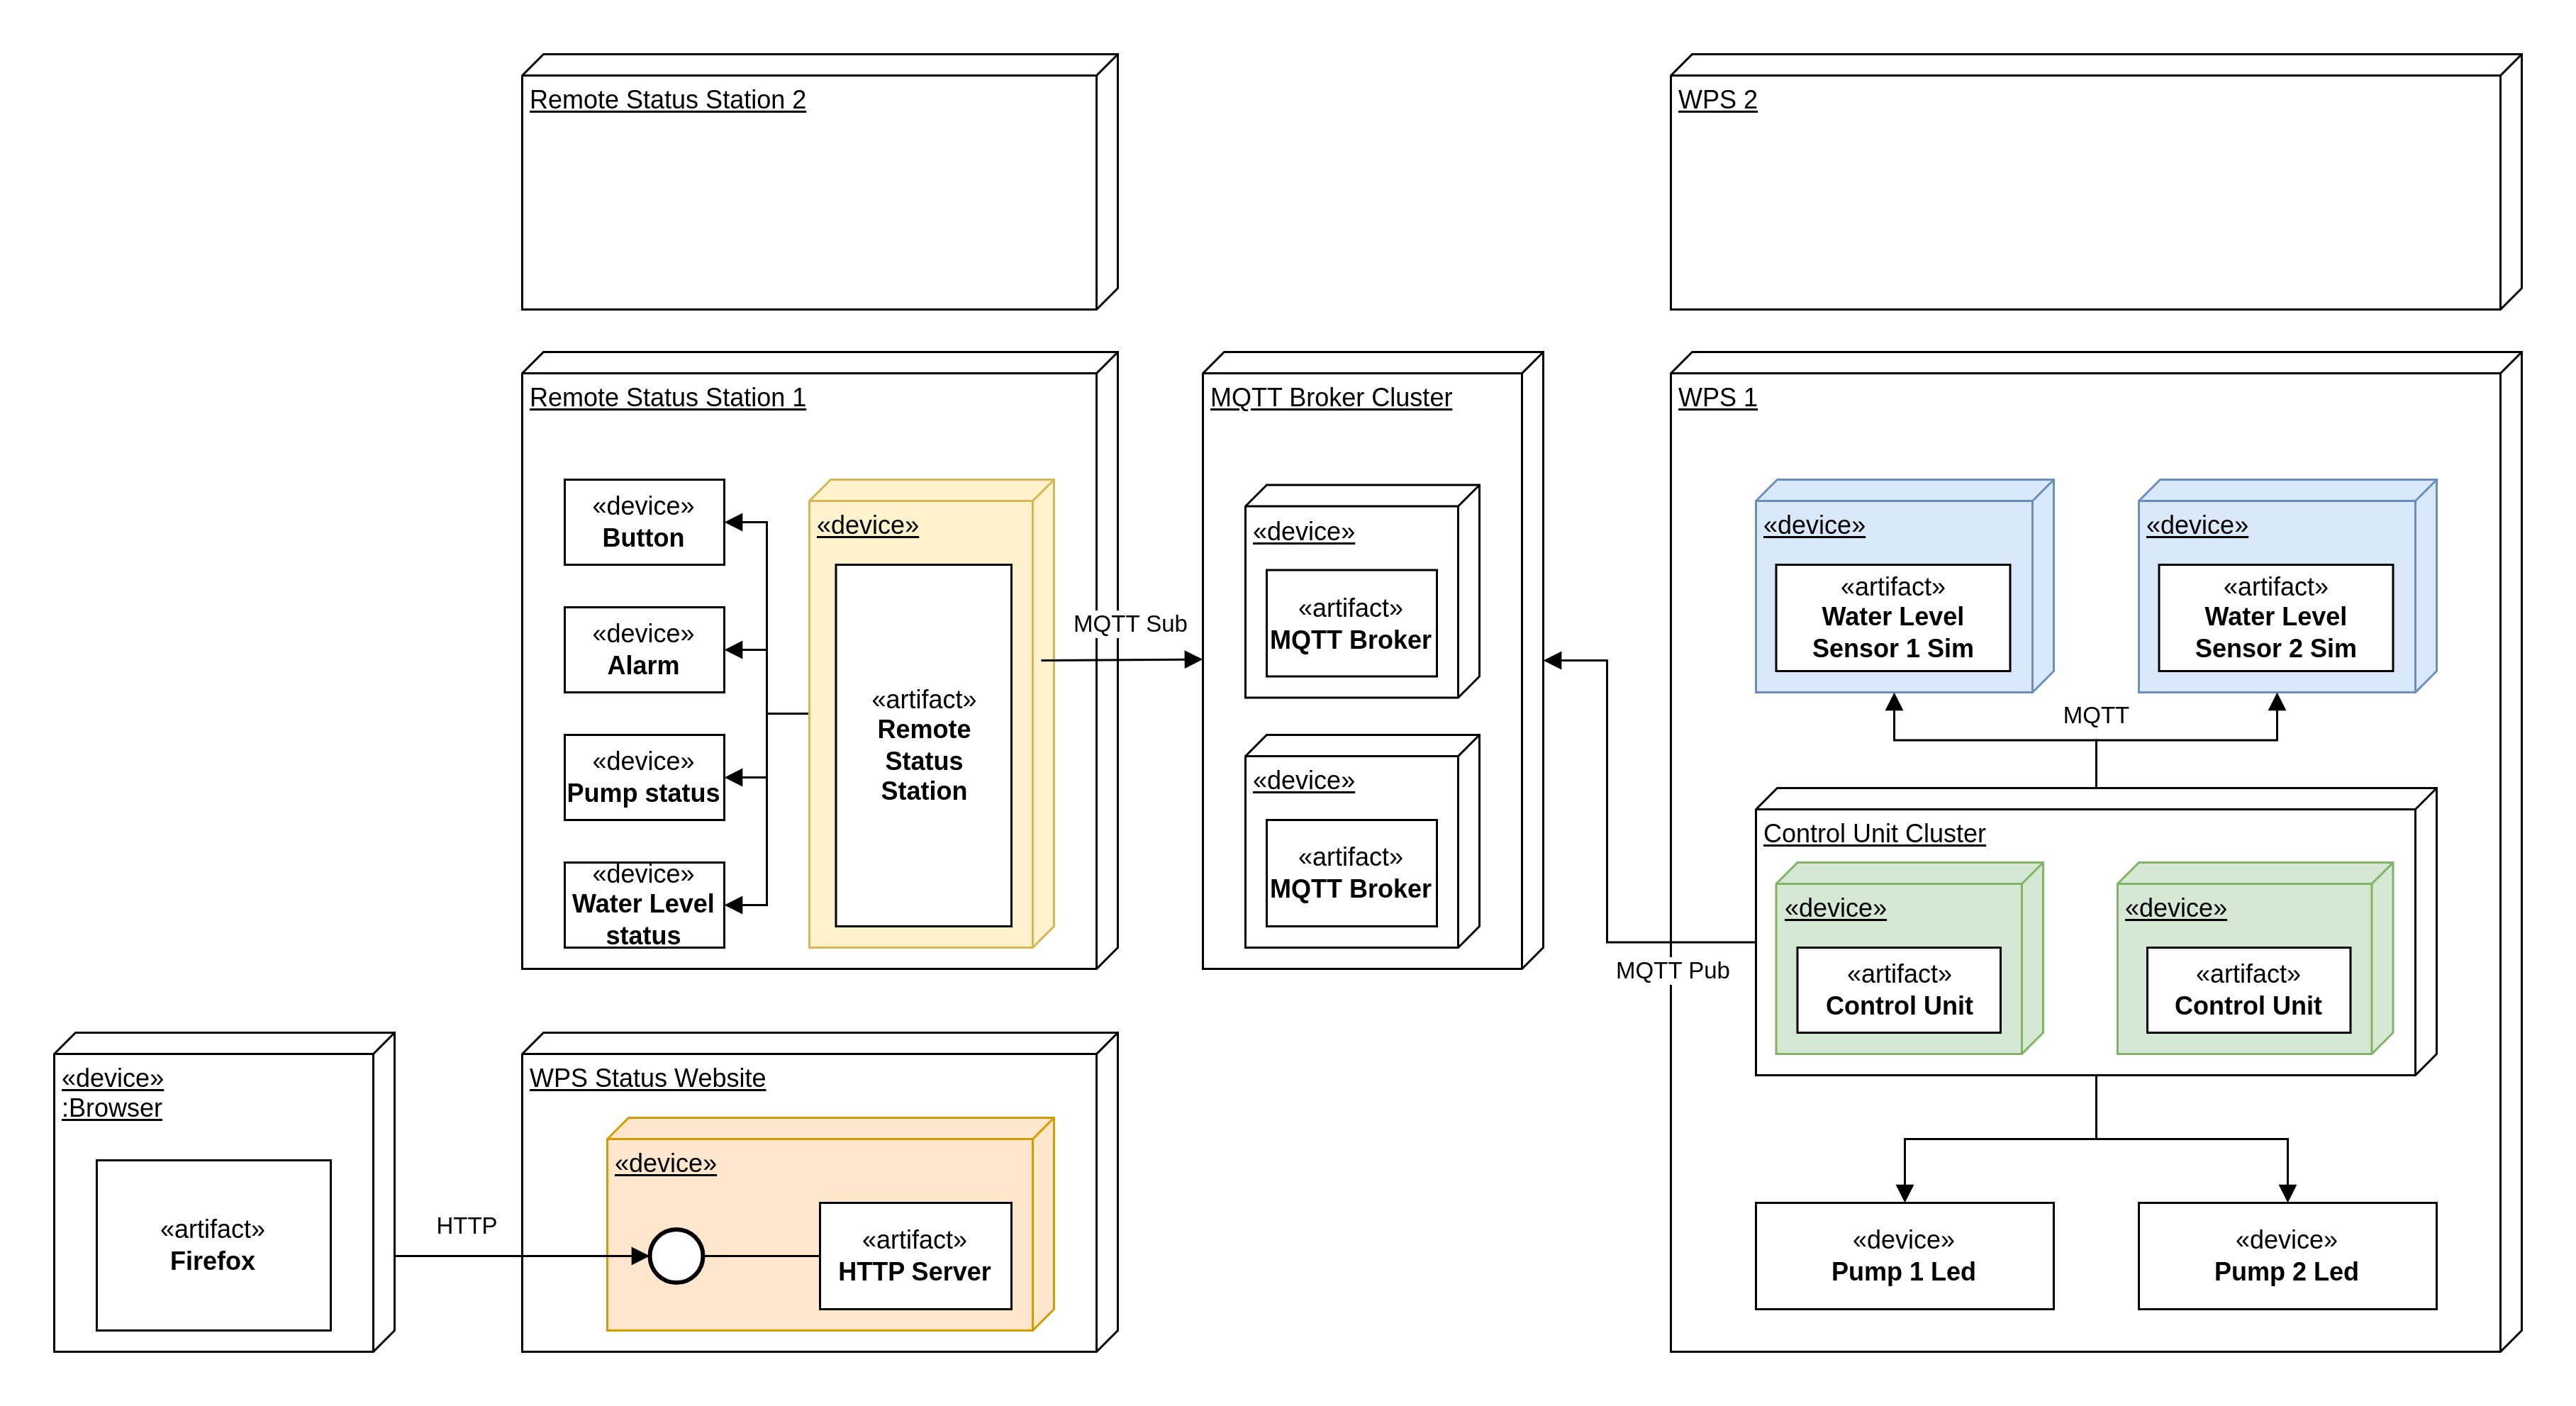
\includegraphics[width=\linewidth]{../diagrams/deployment-diagram-WPS.jpg}
  \caption{Deployment diagram}
  \label{fig:Deployment Diagram}
\end{figure}

\begin{figure}[H]
  \centering
  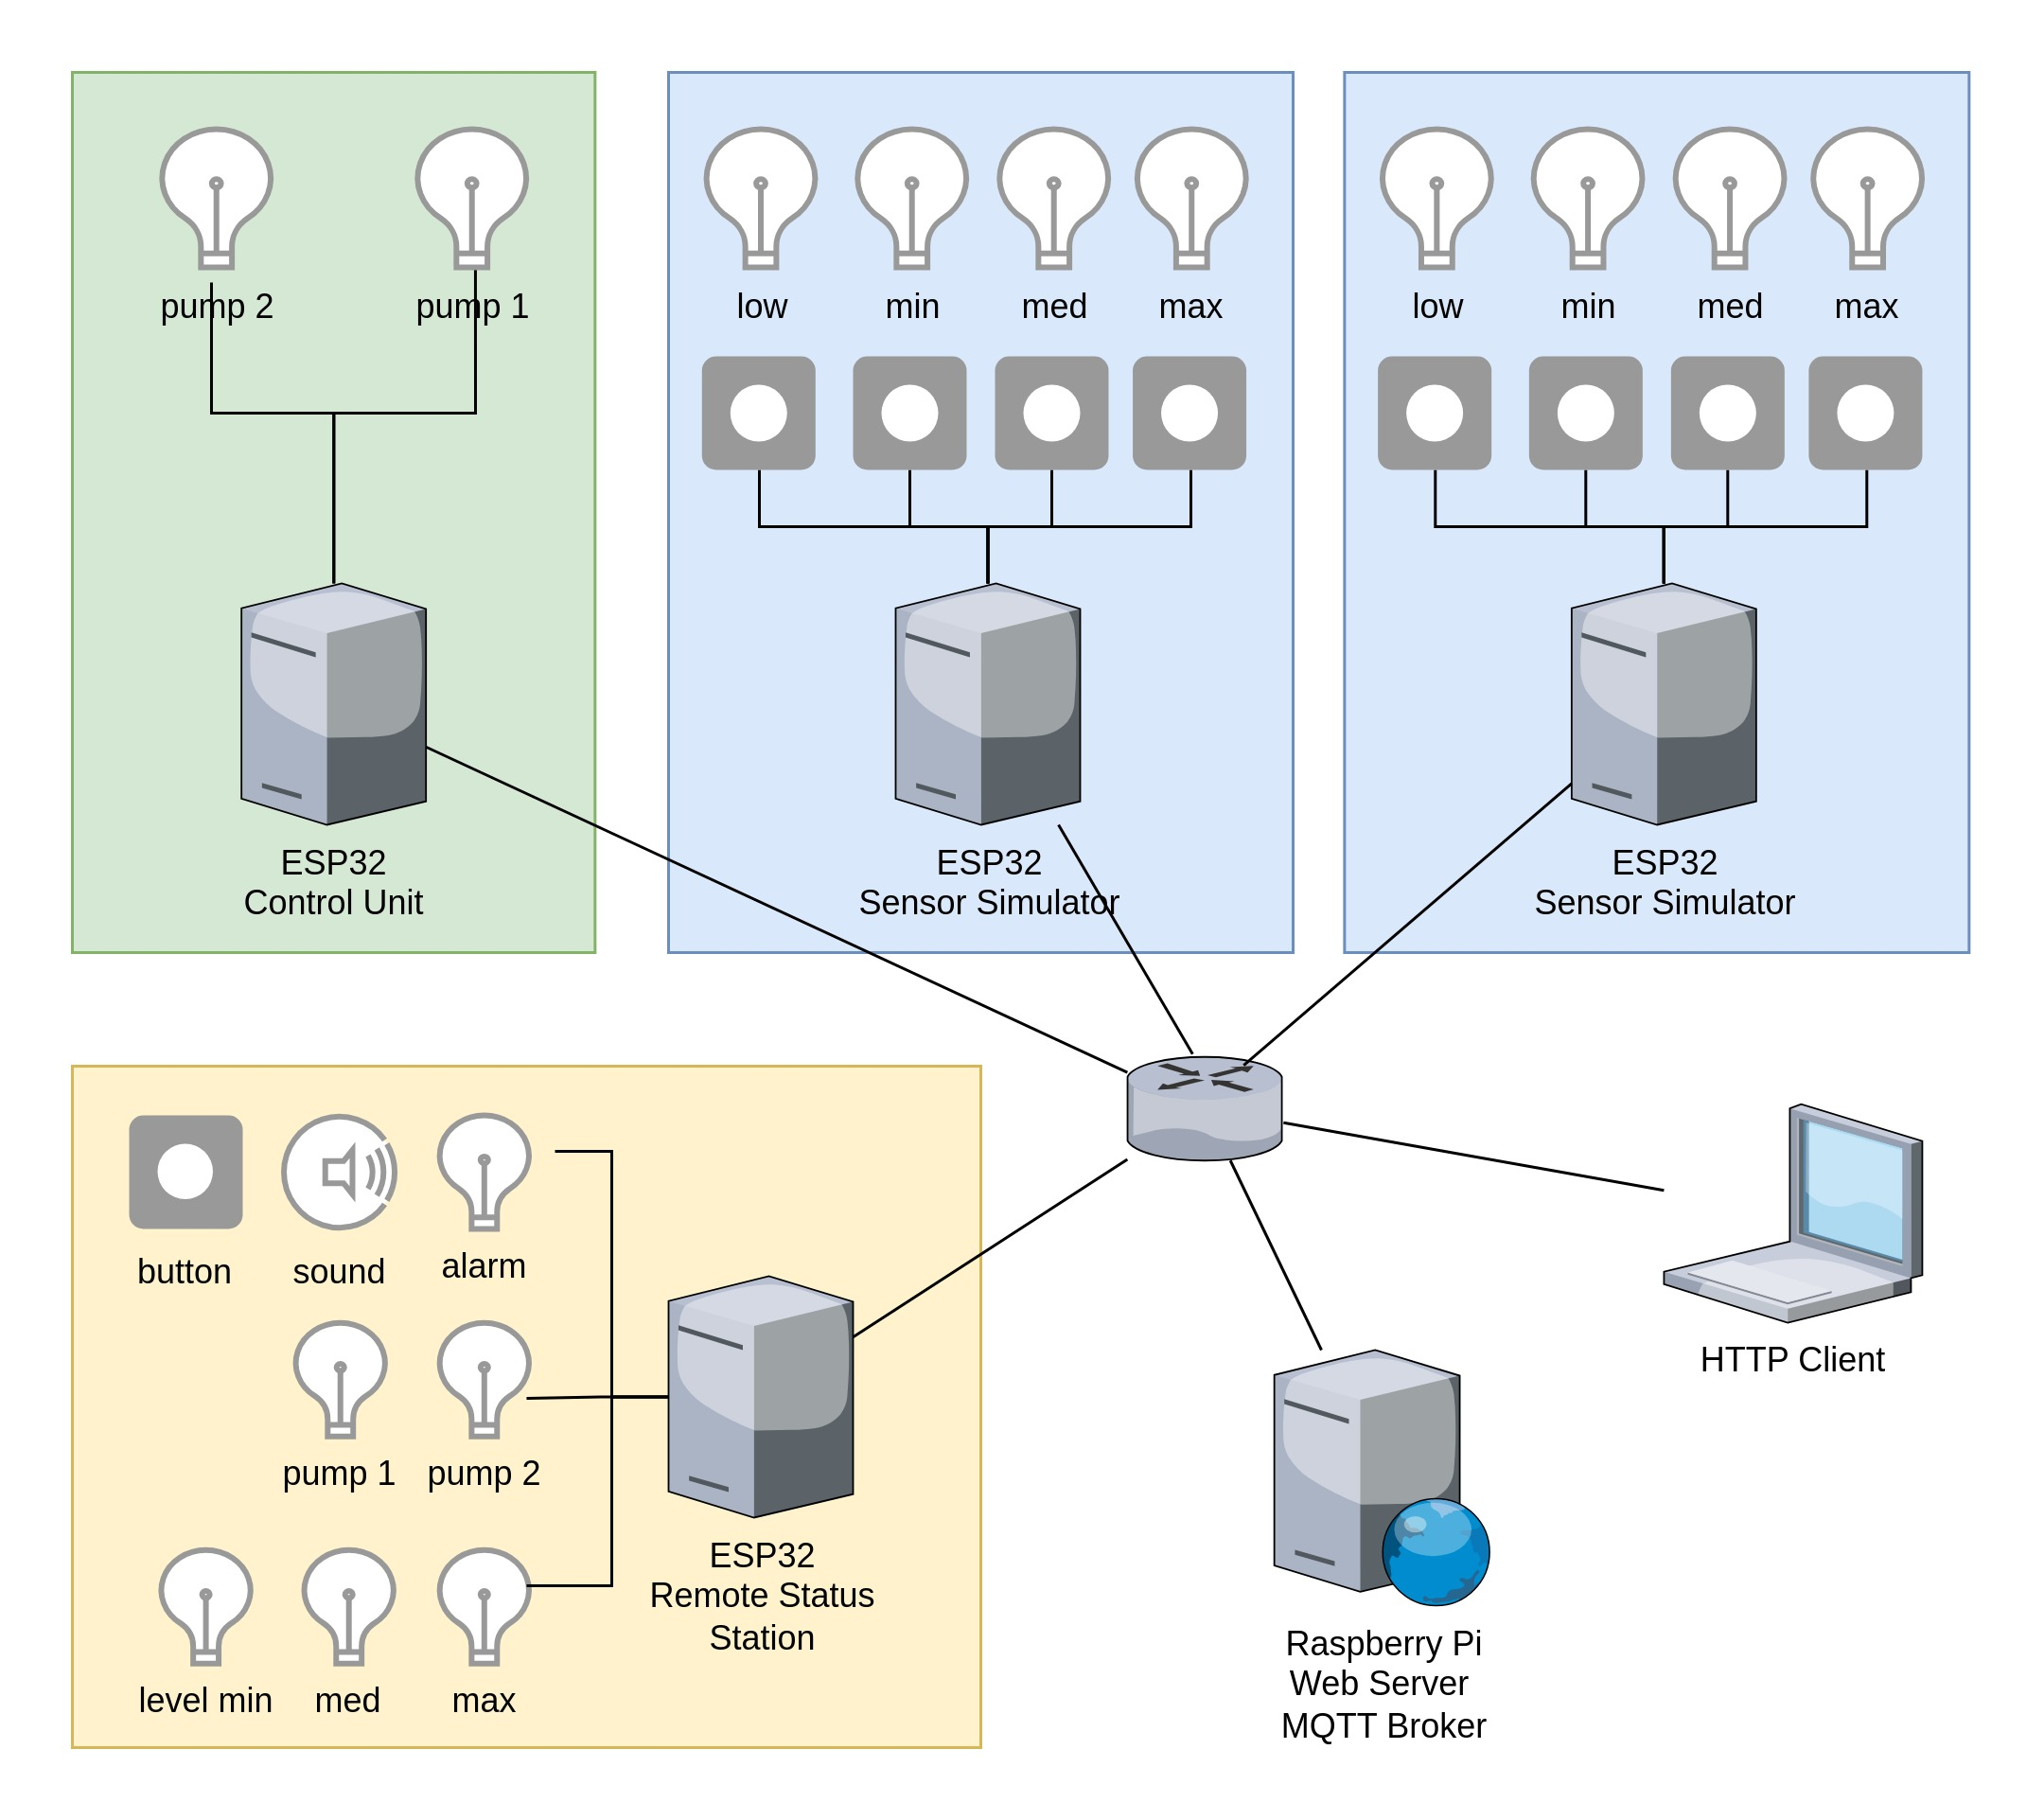
\includegraphics[width=300px]{../diagrams/network-diagram-WPS.jpg}
  \caption{Network diagram}
  \label{fig:Network1 Diagram}
\end{figure}

\end{document}
